% ############### 2.5) COMPONENT INTERFACES ####################

In this section we present the main interfaces used in the system. Given the microservice-based approach, the architecture is composed of many simple components, each one with its own interface (as shown in section 2.2) that handles the basic operations on that specific module. 
\newline
\newline
For simplicity, we decided to explicitly list only the external methods, provided by the API gateway, that ensure the satisfaction of the high-level goals of the different actors.
\newline
\newline
In particular:
\begin{itemize}
    \item UserInterface: it handles the operations of a generic user, such as login, registration and  visualizing and updating account information;
    \item PolicyMakerInterface: it handles the operations of a policy maker, such as visualizing different types of data and statistics, assigning incentives and asking farmers to write good practices;
    \item FarmerInterface: it handles the operations of a farmer, such as visualizing relevant information about his area and production, inserting details about production and problems faced, interacting with other actors through requests and forums and writing good practices; 
    \item AgronomistInterface: it handles the operations of an agronomist, such as managing the areas he is responsible of, visualizing different types of information about the areas and the farmers, answering farmers’ requests and visualizing, updating and confirming the execution of daily plans.
\end{itemize}

\begin{figure}[H]
	\centering
    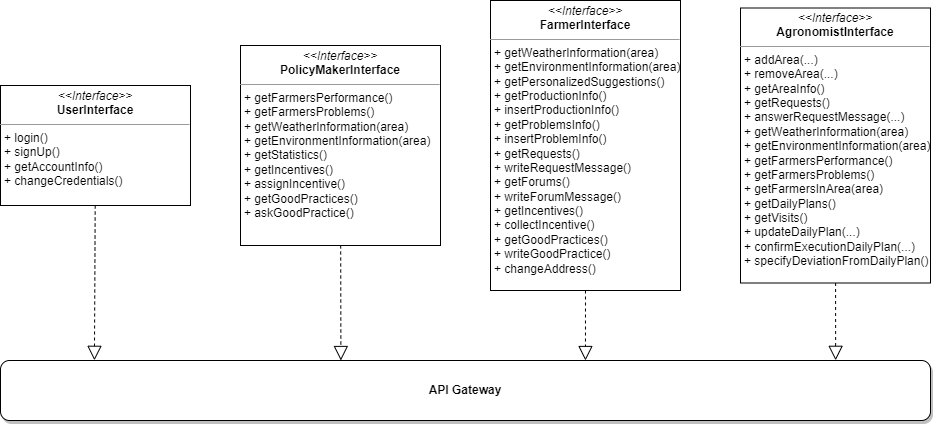
\includegraphics[width=\textwidth]{Images/Architecture/Interface Diagram.png}
	\caption{\label{fig:interfaces_diagram}Interfaces Diagram}
\end{figure}